% Appendix B (single file). Needs only \usepackage{tikz,amsmath,amssymb,booktabs}.
% TikZ styles used by the figures:
\providecommand{\SE}{\Xi}% Born / total self-energy symbol; change here only
\tikzset{
  ret/.style={thick,->},            % retarded line: arrow to the right
  adv/.style={thick,<-},            % advanced line: arrow to the left
  thickline/.style={very thick,->}, % dressed (averaged) line
  thickadv/.style={very thick,<-},
  imp/.style={dashed,thick},        % impurity line = one pairing
  dot/.style={circle,fill,inner sep=1.6pt},
  vert/.style={rectangle,fill,inner sep=2.2pt}, % current vertex v_x
  lab/.style={font=\small}
}

\newpage
\section*{Appendix B: Diagrammatic formulation of disorder averaging}
\label{app:disorder}

\noindent
The objective of this appendix is to establish the disorder-averaging
rules and to identify the diagrammatic channels (dressed bubble,
uncrossed ladder, maximally crossed series) whose sums are evaluated
later: classes 1 and 2 in Appendix~C and class 3 in the main text.
It covers the averaging rule, the diagram rules, the dressed
propagator, the classes of diagrams in the conductivity bubble, and
the definition of the dressed bubble. The route follows
Refs.~\cite{BruusFlensberg,Coleman2015}. Notation: $\hbar=1$,
$\xi_{\mathbf k}=\epsilon_{\mathbf k}-E_{\mathrm F}$, and
$\nu(\epsilon)$ is the density of states per spin and per volume.

\subsection*{B.1\quad Disorder model and Gaussian averaging}

The impurity potential $U(\mathbf r)$ is static, statistically
homogeneous, with zero mean, and Gaussian, so it is fully specified
by its pair correlator. We use white noise,
\[
\overline{U(\mathbf r)}=0,\qquad
\overline{U(\mathbf r)\,U(\mathbf r')}
=W_0\,\delta(\mathbf r-\mathbf r').
\]
For a Gaussian distribution the average of a product of $U$'s
vanishes if the number of factors is odd, and for an even number
it is the sum over all ways of pairing the factors (Wick's theorem
for the disorder), each pair replaced by the correlator. In the
plane-wave basis, with
$\langle\mathbf r|\mathbf k\rangle
=e^{\mathrm{i}\mathbf k\cdot\mathbf r}/\sqrt V$,
\[
U_{\mathbf a\mathbf b}
=\frac1V\int\mathrm{d}^dr\;
e^{-\mathrm{i}(\mathbf a-\mathbf b)\cdot\mathbf r}\,
U(\mathbf r),
\]
and averaging two of them,
\[
\begin{aligned}
\overline{U_{\mathbf a\mathbf b}U_{\mathbf c\mathbf d}}
&=\frac{W_0}{V^2}\int\mathrm{d}^dr\,
e^{-\mathrm{i}(\mathbf a-\mathbf b+\mathbf c-\mathbf d)
\cdot\mathbf r}\\
&=\frac{W_0}{V}\,
\delta_{\mathbf a-\mathbf b,\;\mathbf d-\mathbf c}.
\end{aligned}
\]
The Kronecker delta is momentum conservation: the two impurity
events transfer equal and opposite momenta.

\subsection*{B.2\quad Diagram rules and the Green-function expansion}

For one fixed sample the identity
$G=g_0+g_0UG$, with
$g_0^{R/A}=(E-h_0\pm\mathrm{i}0^+)^{-1}$ and
$h_0=p^2/2m$, gives the successive-scattering series
\[
G^{R/A}
=g_0^{R/A}
+g_0^{R/A}Ug_0^{R/A}
+g_0^{R/A}Ug_0^{R/A}Ug_0^{R/A}
+\cdots ,
\]
in which every $U$ is the same potential. In the plane-wave basis
$g_0(\mathbf k)=(E-\epsilon_{\mathbf k}\pm\mathrm{i}0^+)^{-1}$
is diagonal, $U_{\mathbf k\mathbf p}
=\langle\mathbf k|U|\mathbf p\rangle$ scatters an electron from
$\mathbf p$ to $\mathbf k$, and the $n$th term is
\[
\begin{aligned}
G^{(n)}(\mathbf k,\mathbf k')
={}&\sum_{\mathbf p_1,\dots,\mathbf p_{n-1}}
g_0(\mathbf k)U_{\mathbf k\mathbf p_1}
g_0(\mathbf p_1)U_{\mathbf p_1\mathbf p_2}
\cdots\\
&\qquad\qquad\cdots
U_{\mathbf p_{n-1}\mathbf k'}g_0(\mathbf k').
\end{aligned}
\]
Each term is drawn with the four elements of
Fig.~\ref{fig:dictionary}: a solid line for a clean propagator,
a dot for one factor $U$, a dashed line for the Gaussian pairing
of two dots (weight $W_0/V$ with the momentum condition above),
and a square for the velocity vertex $v_x$. The dashed line is a
bookkeeping device for the average of two impurity events; it is
not a separate physical interaction.

% ===== Figure 1: the dictionary ===================================
\begin{figure}[ht]
\centering
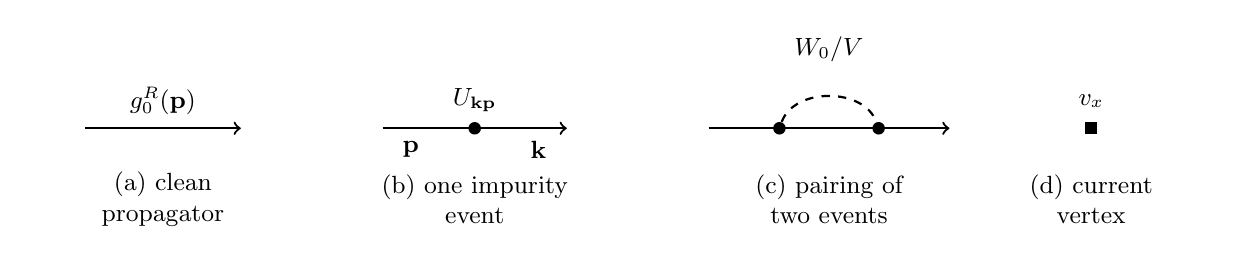
\begin{tikzpicture}[scale=0.9,capt/.style={font=\small,align=center,text width=3.2cm}]
 % (a) clean propagator
 \draw[ret] (0,0)--(2.2,0);
 \node[lab,above] at (1.1,0.05) {$g_0^{R}(\mathbf p)$};
 \node[capt] at (1.1,-1.0) {(a) clean\\ propagator};
 % (b) one factor of U
 \draw[ret] (4.2,0)--(6.8,0);
 \node[dot] at (5.5,0) {};
 \node[lab,below] at (4.6,-0.05) {$\mathbf p$};
 \node[lab,below] at (6.4,-0.05) {$\mathbf k$};
 \node[lab,above] at (5.5,0.1) {$U_{\mathbf k\mathbf p}$};
 \node[capt] at (5.5,-1.0) {(b) one impurity\\ event};
 % (c) a pairing
 \draw[ret] (8.8,0)--(12.2,0);
 \node[dot] (p1) at (9.8,0) {};
 \node[dot] (p2) at (11.2,0) {};
 \draw[imp] (p1) to[bend left=70] (p2);
 \node[lab,above] at (10.5,0.8) {$W_0/V$};
 \node[capt] at (10.5,-1.0) {(c) pairing of\\ two events};
 % (d) vertex
 \node[vert] at (14.2,0) {};
 \node[lab,above] at (14.2,0.15) {$v_x$};
 \node[capt] at (14.2,-1.0) {(d) current\\ vertex};
\end{tikzpicture}
\caption{Rules used to draw the terms of the expansion: (a) a solid
segment is a clean propagator, (b) a dot is one factor of the
impurity potential, which scatters the electron from $\mathbf p$
to $\mathbf k$, (c) a dashed line joins two dots and stands for
their disorder average, with weight $W_0/V$ and momentum
conservation, (d) a square is the current vertex $v_x$.}
\label{fig:dictionary}
\end{figure}


\subsection*{B.3\quad Averaging a single Green function: the Born approximation}

\emph{Order one} has a single $U$ and averages to zero, since
$\overline U=0$. \emph{Order two} is the term of B.2 with $n=2$,
\[
G^{(2)}(\mathbf k,\mathbf k')
=\sum_{\mathbf p}
g_0(\mathbf k)\,U_{\mathbf k\mathbf p}\,
g_0(\mathbf p)\,U_{\mathbf p\mathbf k'}\,
g_0(\mathbf k').
\]
The propagators $g_0$ are not random, so only the two $U$'s are
averaged. By the pair rule of B.1,
\[
\overline{U_{\mathbf k\mathbf p}U_{\mathbf p\mathbf k'}}
=\frac{W_0}{V}\,
\delta_{\mathbf k-\mathbf p,\;\mathbf k'-\mathbf p},
\]
and the delta forces $\mathbf k'=\mathbf k$ while leaving
$\mathbf p$ free:
\[
\begin{aligned}
\overline{G^{(2)}(\mathbf k,\mathbf k')}
&=\sum_{\mathbf p}g_0(\mathbf k)\,
\frac{W_0}{V}\delta_{\mathbf k\mathbf k'}\,
g_0(\mathbf p)g_0(\mathbf k')\\
&=\delta_{\mathbf k\mathbf k'}\;
g_0(\mathbf k)
\left[\frac{W_0}{V}\sum_{\mathbf p}g_0(\mathbf p)\right]
g_0(\mathbf k).
\end{aligned}
\]
The bracket does not depend on $\mathbf k$. We call it the Born
self-energy and write
\[
\SE^{R/A}=\frac{W_0}{V}\sum_{\mathbf p}g_0^{R/A}(\mathbf p),
\qquad\text{so}\qquad
\overline{G^{(2)}(\mathbf k,\mathbf k')}
=\delta_{\mathbf k\mathbf k'}\;
g_0(\mathbf k)\,\SE\,g_0(\mathbf k).
\]
This is an arc: a dashed line joining two dots of the same line.
\emph{Order four} has three pairings of the dots
$d_1,\dots,d_4$, drawn in Fig.~\ref{fig:arcs}:
\begin{itemize}
 \item $(d_1d_2)(d_3d_4)$: two arcs in series, giving
 $g_0\SE g_0\SE g_0$;
 \item $(d_1d_4)(d_2d_3)$: nested arcs, an arc whose internal
 propagator carries a second arc;
 \item $(d_1d_3)(d_2d_4)$: crossed arcs, with internal momenta
 related by
 $\mathbf p_3=\mathbf k-\mathbf p_1+\mathbf p_2$.
\end{itemize}

% ===== Figure 2: averaging a single line ==========================
\begin{figure}[ht]
\centering
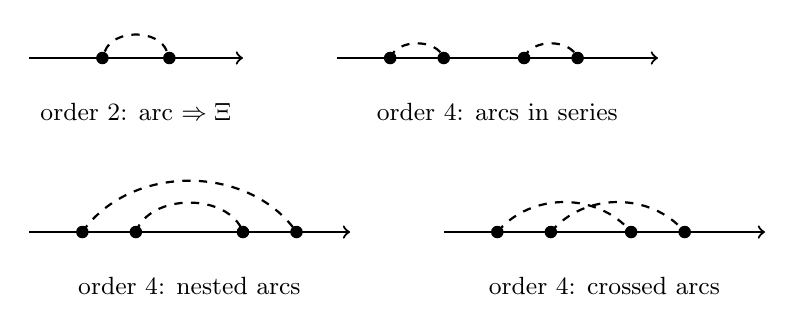
\begin{tikzpicture}[scale=0.85]
 % order 2: arc
 \draw[ret] (0,0)--(3.2,0);
 \node[dot] (a1) at (1.1,0) {};
 \node[dot] (a2) at (2.1,0) {};
 \draw[imp] (a1) to[bend left=70] (a2);
 \node[lab] at (1.6,-0.8) {order 2: arc $\Rightarrow\SE$};
 % order 4: series
 \draw[ret] (4.6,0)--(9.4,0);
 \foreach \x in {5.4,6.2,7.4,8.2}{\node[dot] at (\x,0) {};}
 \draw[imp] (5.4,0) to[bend left=70] (6.2,0);
 \draw[imp] (7.4,0) to[bend left=70] (8.2,0);
 \node[lab] at (7.0,-0.8) {order 4: arcs in series};
 % nested
 \draw[ret] (0,-2.6)--(4.8,-2.6);
 \foreach \x in {0.8,1.6,3.2,4.0}{\node[dot] at (\x,-2.6) {};}
 \draw[imp] (0.8,-2.6) to[bend left=55] (4.0,-2.6);
 \draw[imp] (1.6,-2.6) to[bend left=70] (3.2,-2.6);
 \node[lab] at (2.4,-3.4) {order 4: nested arcs};
 % crossed
 \draw[ret] (6.2,-2.6)--(11,-2.6);
 \foreach \x in {7.0,7.8,9.0,9.8}{\node[dot] at (\x,-2.6) {};}
 \draw[imp] (7.0,-2.6) to[bend left=50] (9.0,-2.6);
 \draw[imp] (7.8,-2.6) to[bend left=50] (9.8,-2.6);
 \node[lab] at (8.6,-3.4) {order 4: crossed arcs};
\end{tikzpicture}
\caption{Average of a single Green function. Order 2 gives one
arc, which defines the Born self-energy $\SE$. Of the three
pairings at order 4, the series of arcs is a repeated use of
$\SE$, the nested arcs belong to the exact self-energy but are
not evaluated here, and the crossed arcs are suppressed by a
power of $1/k_{\mathrm F}\ell$.}
\label{fig:arcs}
\end{figure}


Every term is a chain of irreducible blocks, so the average obeys
a Dyson equation,
\[
\overline{G}^{R/A}(\mathbf k)
=g_0^{R/A}(\mathbf k)
+g_0^{R/A}(\mathbf k)\,
\SE^{R/A}_{\mathrm{tot}}(\mathbf k)\,
\overline{G}^{R/A}(\mathbf k)
\;\Longrightarrow\;
\overline{G}^{R/A}(\mathbf k)
=\frac{1}{E-\epsilon_{\mathbf k}
-\SE^{R/A}_{\mathrm{tot}}(\mathbf k)}.
\]
In the Born approximation we keep only the single arcs, which
gives $\SE_{\mathrm{tot}}\simeq\SE$, i.e., built from the bare
$g_0$. The nested arcs belong to the exact
$\SE_{\mathrm{tot}}$ and are not evaluated. For a constant density
of states over a bandwidth much larger than $\gamma$, replacing
the internal $g_0$ by $\overline G$ (the self-consistent Born
approximation) leaves the leading $\operatorname{Im}\SE$
unchanged. In the weak-disorder regime $k_{\mathrm F}\ell\gg1$
we keep only the non-crossing Born term; crossed arcs are smaller
by a power of $1/k_{\mathrm F}\ell$ (a phase-space argument, see
Fig.~11.6 of Ref.~\cite{BruusFlensberg}), which we quote and do
not derive, and they are neglected.

\paragraph{Born self-energy and scattering time.}
Trading the momentum sum for an energy integral,
\[
\SE^{R}(E)
=W_0\!\int\!\mathrm{d}\epsilon\,
\frac{\nu(\epsilon)}{E-\epsilon+\mathrm{i}0^+}
=W_0\,\mathcal P\!\!\int\!\mathrm{d}\epsilon\,
\frac{\nu(\epsilon)}{E-\epsilon}
-\mathrm{i}\pi W_0\,\nu(E).
\]
The real part depends on the high-energy cutoff of the continuum
model; for a slowly varying density of states it is approximately
constant near the Fermi energy and is absorbed into the chemical
potential. For white noise $\SE$ depends on $E$ and not on
$\mathbf k$, so we write
\[
\SE^{R/A}=\mp\frac{\mathrm{i}}{2\tau},\qquad
\frac1\tau=2\pi W_0\,\nu_{\mathrm F},\qquad
\gamma\equiv\frac1{2\tau}
=\pi W_0\,\nu_{\mathrm F},
\]
and at $E=E_{\mathrm F}$
\[
\overline G^{R/A}(\mathbf k)
=\frac{1}{-\xi_{\mathbf k}\pm\mathrm{i}\gamma},
\qquad
\overline G^R\overline G^A
=\frac{1}{\xi_{\mathbf k}^2+\gamma^2}.
\]
The infinitesimal $0^+$ of the bare propagators has been replaced
by the finite width $\gamma$.

The two poles of $\overline G^R\overline G^A$ lie at
$\xi=\pm\mathrm{i}\gamma$, on opposite sides of the real axis, and
\[
\int_{-\infty}^{\infty}\mathrm{d}\xi\;
\overline G^R\,\overline G^A
=\frac{\pi}{\gamma}=2\pi\tau.
\]
We say that such a pair of propagators is \emph{pinched}: as
$\gamma\to0$ the poles approach the real axis from opposite sides,
the integration contour is trapped between them, and the
integral grows as $1/\gamma$. For two retarded functions both
poles lie in the same half-plane, so the contour can be closed on
the other side, where there is no pole, and
\[
\int_{-\infty}^{\infty}\mathrm{d}\xi\;
\big(\overline G^R\big)^2=0,
\]
and likewise for two advanced functions: there is no pinch. This
holds for a constant density of states and an infinite band; for
a finite band the same-side integrals are of order $1/E_{\mathrm F}$,
smaller than the pinched one by a factor of order
$\gamma/E_{\mathrm F}$. This is the contour argument for the
dominance of the retarded--advanced term near the Fermi surface
used in the main text.

\subsection*{B.4\quad Diagram classes in the conductivity bubble}

The conductivity contains the \emph{product} of a retarded and an
advanced Green function of the same sample. Both depend on the
same $U$, so their average does not factorise,
\[
\overline{G^R(\mathbf k,\mathbf k')\,
G^A(\mathbf k',\mathbf k)}
\neq
\overline{G^R(\mathbf k,\mathbf k')}\;
\overline{G^A(\mathbf k',\mathbf k)},
\]
and the difference between the two sides is exactly what the
diagrams below will supply. Exactly, \emph{every} Gaussian pairing
of the dots on the two lines contributes; the work below is to
decide which families of pairings dominate. Drawing the two lines
closed into a loop by the current vertices, with the retarded
line on top and the advanced line below, a pairing can join two
dots of the same line (an \emph{arc}) or one dot of each line
(a \emph{rung}).

\paragraph{Lowest orders.}
With $N=2$ dots there are three diagrams
(Fig.~\ref{fig:lowest}): an arc on the retarded line, an arc on
the advanced line, or one rung. With $N=4$ and two dots on each
line there are three pairings (Fig.~\ref{fig:classes}): an arc on
each line, two uncrossed rungs, and two crossed rungs. To describe
the $N=4$ pairings we name the dots by their position, from the
left: $u_1,u_2$ on the retarded (upper) line and $l_1,l_2$ on the
advanced (lower) line, as in Fig.~\ref{fig:classes}. The electron
enters the loop at the left current vertex with momentum
$\mathbf k$ and leaves at the right vertex with $\mathbf k'$.
On the retarded line it runs to the right, so $u_1$ takes
$\mathbf k\to\mathbf p$ and $u_2$ takes $\mathbf p\to\mathbf k'$,
that is $u_1=U_{\mathbf p\mathbf k}$,
$u_2=U_{\mathbf k'\mathbf p}$ (recall that
$U_{\mathbf a\mathbf b}$ scatters $\mathbf b\to\mathbf a$).
The advanced line runs to the left, so from the right vertex it
meets $l_2$ first ($\mathbf k'\to\mathbf a$) and then $l_1$
($\mathbf a\to\mathbf k$):
$l_2=U_{\mathbf a\mathbf k'}$,
$l_1=U_{\mathbf k\mathbf a}$. Here $\mathbf a$ is the momentum
of the advanced line between its two dots. A pairing is named by
the dots it joins: $(u_1l_1)$ is a dashed line from the upper
left dot to the lower left dot. The pair rule of B.1 says that
the momenta transferred at the two paired dots are equal and
opposite, where the transfer at a dot is out minus in
($\mathbf p-\mathbf k$ at $u_1$,
$\mathbf k'-\mathbf p$ at $u_2$,
$\mathbf k-\mathbf a$ at $l_1$,
$\mathbf a-\mathbf k'$ at $l_2$). This fixes $\mathbf a$:
\begin{align*}
&\text{uncrossed } (u_1l_1)(u_2l_2):
\quad
(\mathbf p-\mathbf k)+(\mathbf k-\mathbf a)=0
\ \Rightarrow\ \mathbf a=\mathbf p,\\
&\text{crossed } (u_1l_2)(u_2l_1):
\quad
(\mathbf p-\mathbf k)+(\mathbf a-\mathbf k')=0
\ \Rightarrow\ \mathbf a=\mathbf K-\mathbf p,
\quad \mathbf K=\mathbf k+\mathbf k'.
\end{align*}
(The second pair of each line gives the same $\mathbf a$.)
So the two lines carry the same momentum between uncrossed
rungs, and opposite momenta, up to the constant $\mathbf K$,
between crossed rungs.

\paragraph{Why $\mathbf K\to0$.}
In the uncrossed diagram the loop sum is over
$\overline G^R(\mathbf p)\,\overline G^A(\mathbf p)$: the two
propagators have the same energy $\xi_{\mathbf p}$ for every
$\mathbf p$, so their poles always face each other and the sum
is pinched (B.3). In the crossed diagram the sum is over
$\overline G^R(\mathbf p)\,\overline G^A(\mathbf K-\mathbf p)$,
and the two energies differ. For small $\mathbf K$, using
$\epsilon_{-\mathbf p}=\epsilon_{\mathbf p}$,
\[
\xi_{\mathbf K-\mathbf p}
=\xi_{\mathbf p-\mathbf K}
\simeq\xi_{\mathbf p}-\delta,
\qquad
\delta=\mathbf v_{\mathbf p}\cdot\mathbf K,
\]
and the energy integral is
\[
\int\mathrm d\xi\,
\frac{1}{(-\xi+\mathrm i\gamma)
(-\xi+\delta-\mathrm i\gamma)}
=\frac{\pi}{\gamma+\mathrm i\delta/2}.
\]
This equals the pinched value $\pi/\gamma$ at $\delta=0$ and
falls off once $|\delta|\gtrsim\gamma$, that is
$v_{\mathrm F}K\gtrsim1/2\tau$, or
$K\gtrsim1/2\ell$. So ``$\mathbf K\to0$'' means
$K\lesssim1/\ell$. Since $\mathbf K=\mathbf k+\mathbf k'$ is
the sum of the momenta at the two current vertices, this says
$\mathbf k'\approx-\mathbf k$: the electron leaves the loop
moving backwards. Physically, the advanced line is the complex
conjugate amplitude, and the crossed diagram pairs a path with
its time-reversed partner, which have the same phase only if
$\mathbf k'=-\mathbf k$.

% ===== Figure: lowest order =====
\begin{figure}[ht]
\centering
\begin{tikzpicture}[scale=0.78]
 \newcommand{\frmlow}{
   \draw[ret] (0,0)--(4.6,0);
   \draw[adv] (0,-1.4)--(4.6,-1.4);
   \draw[gray] (0,0)--(0,-1.4);
   \draw[gray] (4.6,0)--(4.6,-1.4);
   \node[vert] at (0,-0.7) {};
   \node[vert] at (4.6,-0.7) {};
 }
 \begin{scope}
  \frmlow
  \node[dot] (a) at (1.5,0) {};
  \node[dot] (b) at (3.1,0) {};
  \draw[imp] (a) to[bend left=70] (b);
  \node[lab] at (2.3,-2.3) {arc on the retarded line};
 \end{scope}
 \begin{scope}[xshift=6.4cm]
  \frmlow
  \node[dot] at (2.3,0) {};
  \node[dot] at (2.3,-1.4) {};
  \draw[imp] (2.3,0)--(2.3,-1.4);
  \node[lab] at (2.3,-2.3) {one rung};
 \end{scope}
 \begin{scope}[xshift=12.8cm]
  \frmlow
  \node[dot] (a) at (1.5,-1.4) {};
  \node[dot] (b) at (3.1,-1.4) {};
  \draw[imp] (a) to[bend right=70] (b);
  \node[lab] at (2.3,-2.3) {arc on the advanced line};
 \end{scope}
\end{tikzpicture}
\caption{The three diagrams with $N=2$ dots.}
\label{fig:lowest}
\end{figure}

% ===== Figure 4: the three classes at fourth order ================
\begin{figure}[ht]
\centering
\begin{tikzpicture}[scale=0.9]
 \newcommand{\nodelab}{
   \node[lab,anchor=north east,inner sep=1pt] at (1.25,-0.05) {$u_1$};
   \node[lab,anchor=north west,inner sep=1pt] at (2.55,-0.05) {$u_2$};
   \node[lab,anchor=south east,inner sep=1pt] at (1.25,-1.35) {$l_1$};
   \node[lab,anchor=south west,inner sep=1pt] at (2.55,-1.35) {$l_2$};
   \node[lab,above] at (0.35,0.05) {$\mathbf k$};
   \node[lab,above] at (3.45,0.05) {$\mathbf k'$};
 }

 % class 1 : arcs on each line
 \begin{scope}
  \draw[ret] (0,0)--(3.8,0);
  \draw[adv] (0,-1.4)--(3.8,-1.4);
  \draw[gray] (0,0)--(0,-1.4);
  \draw[gray] (3.8,0)--(3.8,-1.4);
  \node[vert] at (0,-0.7) {};
  \node[vert] at (3.8,-0.7) {};
  \node[dot] (u1) at (1.3,0) {};
  \node[dot] (u2) at (2.5,0) {};
  \node[dot] (l1) at (1.3,-1.4) {};
  \node[dot] (l2) at (2.5,-1.4) {};
  \draw[imp] (u1) to[bend left=70] (u2);
  \draw[imp] (l1) to[bend right=70] (l2);
  \nodelab
  \node[lab] at (1.9,-3.0) {\textbf{class 1}: arcs on each line};
 \end{scope}

 % class 2 : uncrossed rungs
 \begin{scope}[xshift=5.4cm]
  \draw[ret] (0,0)--(3.8,0);
  \draw[adv] (0,-1.4)--(3.8,-1.4);
  \draw[gray] (0,0)--(0,-1.4);
  \draw[gray] (3.8,0)--(3.8,-1.4);
  \node[vert] at (0,-0.7) {};
  \node[vert] at (3.8,-0.7) {};
  \node[dot] (u1) at (1.3,0) {};
  \node[dot] (u2) at (2.5,0) {};
  \node[dot] (l1) at (1.3,-1.4) {};
  \node[dot] (l2) at (2.5,-1.4) {};
  \draw[imp] (u1)--(l1);
  \draw[imp] (u2)--(l2);
  \nodelab
  \node[lab,above] at (1.9,0.35) {$\mathbf p$};
  \node[lab,below] at (1.9,-1.75) {$\mathbf p=\mathbf a$};
  \node[lab] at (1.9,-3.0) {\textbf{class 2}: uncrossed rungs};
 \end{scope}

 % class 3 : crossed rungs
 \begin{scope}[xshift=10.8cm]
  \draw[ret] (0,0)--(3.8,0);
  \draw[adv] (0,-1.4)--(3.8,-1.4);
  \draw[gray] (0,0)--(0,-1.4);
  \draw[gray] (3.8,0)--(3.8,-1.4);
  \node[vert] at (0,-0.7) {};
  \node[vert] at (3.8,-0.7) {};
  \node[dot] (u1) at (1.3,0) {};
  \node[dot] (u2) at (2.5,0) {};
  \node[dot] (l1) at (1.3,-1.4) {};
  \node[dot] (l2) at (2.5,-1.4) {};
  \draw[imp] (u1)--(l2);
  \draw[imp] (u2)--(l1);
  \nodelab
  \node[lab,above] at (1.9,0.35) {$\mathbf p$};
  \node[lab,below] at (1.9,-1.75) {$\mathbf a=\mathbf K-\mathbf p$};
  \node[lab] at (1.9,-3.0) {\textbf{class 3}: crossed rungs};
 \end{scope}
\end{tikzpicture}
\caption{The three pairings of four dots, two on each line ($N=4$).
The dots are named $u_1,u_2$ (upper line) and $l_1,l_2$ (lower
line) from the left; $\mathbf k,\mathbf k'$ are the momenta at
the two current vertices, $\mathbf p$ is the momentum between
the dots of the upper line and $\mathbf a$ between those of the
lower line. Class~1: every dashed line joins two dots of the
same line. Class~2: dashed lines join the two lines without
crossing, so both lines carry the same momentum $\mathbf p$
between the rungs. Class~3: the dashed lines cross, and the
lower line carries $\mathbf K-\mathbf p$ with
$\mathbf K=\mathbf k+\mathbf k'$ the sum of the momenta at the
two vertices.}
\label{fig:classes}
\end{figure}

\paragraph{Arbitrary order.}
For $N$ dots every pairing is a set of arcs and rungs. An isolated
Born self-energy insertion, containing no nested impurity lines
or rung crossings, is already included in the thick (Born-dressed)
propagator $\overline G$. More complicated nested or crossed
self-energy structures are neglected in the Born approximation.
Within this approximation, the remaining inter-line pairings
form $n$ rungs, whose possible arrangements are now classified.
Number the rungs by the dot they leave on the retarded line,
left to right, and let rung $i$ end on the $\pi(i)$th dot of the
advanced line. The arrangement is the permutation $\pi$ of
$\{1,\dots,n\}$, and there are $n!$ of them. Two of them stand
out (Table~\ref{tab:classes}): $\pi=$ identity, in which no rungs
cross (the ladder), and $\pi=$ reversal, in which every rung
crosses every other (the maximally crossed diagram, whose sum
is the Cooperon of weak localization
\cite[Sec.~15.4]{BruusFlensberg}).

\begin{table}[ht]
\centering
\renewcommand{\arraystretch}{1.25}
\begin{tabular}{@{}p{1.2cm}p{5.2cm}p{7cm}@{}}
\toprule
Class & Pairing structure & Name\\
\midrule
1 & no rung; arcs only & dressed bubble\\
2 & rungs, none crossing & ladder\\
3 & rungs, all crossing each other & maximally crossed series
(Cooperon channel)\\
\bottomrule
\end{tabular}
\caption{Families of diagrams in the retarded--advanced bubble.}
\label{tab:classes}
\end{table}

\paragraph{Which arrangements matter.}
We need a rule for the size of a diagram. Each rung brings a
weight $W_0=1/(2\pi\nu\tau)$ (B.3) and a free momentum sum.
If that sum runs over a pinched retarded--advanced pair carrying
the same momentum $\mathbf p$, as in the ladder, it gives
\[
\frac1V\sum_{\mathbf p}
\overline G^R_{\mathbf p}\overline G^A_{\mathbf p}
\simeq
\nu\int\mathrm{d}\xi\,
\overline G^R\overline G^A
=2\pi\nu\tau,
\]
and the rung costs $W_0\cdot2\pi\nu\tau=1$: it is of order one
however many rungs there are, so a ladder cannot be truncated
and must be summed. In the crossed diagram the pair carries
opposite momenta $\mathbf p$ and $\mathbf K-\mathbf p$, and
for $\mathbf K\to0$ inversion symmetry
$\epsilon_{-\mathbf p}=\epsilon_{\mathbf p}$ turns the sum into
the same integral,
\[
\int\mathrm{d}\xi_{\mathbf p}\,
\overline G^R(\mathbf p)\overline G^A(-\mathbf p)
=
\int\mathrm{d}\xi_{\mathbf p}\,
\overline G^R(\mathbf p)\overline G^A(\mathbf p)
=\frac{\pi}{\gamma}=2\pi\tau,
\]
so the crossed channel is enhanced by the same mechanism, but
only for $\mathbf K\to0$, where
$\overline G^A(\mathbf K-\mathbf p)
\to\overline G^A(-\mathbf p)$. If instead a sum contains no
pinched pair, the energy integral of same-side propagators
vanishes at leading order (B.3), and what survives is smaller
by the ratio
$W_0\nu/E_{\mathrm F}\sim1/(E_{\mathrm F}\tau)
\sim1/k_{\mathrm F}\ell$. This is an order-of-magnitude
estimate, not a calculation of each diagram. The criterion for
keeping the enhancement is therefore: \emph{every rung carries
a pinched retarded--advanced pair, with equal momenta or with
opposite momenta and $\mathbf K\to0$.} It is a necessary
condition for a leading contribution, not a sufficient one,
as the $n=3$ examples show.

Apply it to the $n=3$ arrangements of Fig.~\ref{fig:perm}.
Writing $\mathbf p_0=\mathbf k$, $\mathbf p_1$, $\mathbf p_2$
and $\mathbf p_3=\mathbf k'$ for the retarded momenta and
$\mathbf a_j$ for the advanced momentum between the $j$th and
$(j+1)$th lower dot counted from the left
($\mathbf a_0=\mathbf k$, $\mathbf a_3=\mathbf k'$), the pair
rule fixes the $\mathbf a_j$ in terms of the $\mathbf p_i$,
exactly as for $N=4$ above:
\begin{itemize}
 \item identity:
 $\mathbf a_1=\mathbf p_1$, $\mathbf a_2=\mathbf p_2$,
 so both sums have a pinched pair, for every $\mathbf p$;

 \item reversal:
 $\mathbf a_1=\mathbf K-\mathbf p_2$,
 $\mathbf a_2=\mathbf K-\mathbf p_1$,
 so both sums are pinched for $\mathbf K\to0$;

 \item $(132)$ and $(213)$: a ladder rung next to a crossed pair.
 For $(132)$,
 $\mathbf a_1=\mathbf p_1$ and
 $\mathbf a_2=\mathbf p_1+\mathbf p_3-\mathbf p_2$,
 so both sums are pinched, the second when
 $\mathbf p_1+\mathbf p_3\to0$ (for $(213)$,
 $\mathbf a_1=\mathbf p_0+\mathbf p_2-\mathbf p_1$ and
 $\mathbf a_2=\mathbf p_2$, with
 $\mathbf p_0+\mathbf p_2\to0$); these small combinations are
 themselves integrated over, as $\mathbf K$ is in the crossed
 diagram. The rung touching a current vertex multiplies the
 diagram by
 $\sum_{\mathbf k}v_{\mathbf kx}
 \overline G^R_{\mathbf k}\overline G^A_{\mathbf k}$,
 which vanishes for white noise because the summand is odd
 in $\mathbf k$;

 \item $(231)$ and $(312)$: for $(231)$,
 $\mathbf a_1=\mathbf K-\mathbf p_2$ but
 $\mathbf a_2=\mathbf p_1-\mathbf p_2+\mathbf p_3$,
 which equals no single $\mathbf p_i$, so only one of the two
 sums has a pinched pair; the other is suppressed by a power
 of $1/k_{\mathrm F}\ell$ (the phase-space argument of B.3).
 $(312)$ is its mirror image.
\end{itemize}
For $n=3$, the identity and reversal arrangements retain the
retarded--advanced enhancement throughout and generate the
ladder and maximally crossed families. The two mixed arrangements
also retain the pinch in their sums, but vanish for white-noise
disorder by the odd-velocity symmetry at a current vertex. The
remaining two lose one of the pinched sums. We use this
enumeration to illustrate the selection; we do not claim a
general proof for arbitrary $n$. Arcs that cross a rung
(Fig.~\ref{fig:straddle}) fail the criterion in the same way.

The same vertex factor
$\sum_{\mathbf k}v_{\mathbf kx}
\overline G^R_{\mathbf k}\overline G^A_{\mathbf k}$
also makes every $S^{(n)}_{\mathrm{ladder}}$ with $n\ge1$
vanish for isotropic white noise at $\mathbf q=0$, $\omega=0$,
since in the ladder the first and last pairs touch the vertices.
We still keep the ladder as a family: it is where the vertex
corrections of anisotropic disorder and the diffusion pole at
finite $\mathbf q,\omega$ come from (Appendix~C).

\paragraph{The approximation made.}
We retain the dressed bubble, the ladder and the maximally
crossed series, the families in which every loop keeps the
retarded--advanced enhancement. Arrangements that keep the
enhancement can still vanish by symmetry, as the mixed $n=3$
ones do for white noise. The pairings that lose a pinched sum
are suppressed: the factor $1/k_{\mathrm F}\ell$ above is an
estimate of their typical size, the actual suppression depends
on the diagram, and it is not calculated here.

% ===== Figure: the six arrangements of three rungs =====
\providecommand{\permdiag}[3]{
  \draw[thick,->] (0,0)--(4.6,0);
  \draw[thick,<-] (0,-1.4)--(4.6,-1.4);
  \draw[gray] (0,0)--(0,-1.4);
  \draw[gray] (4.6,0)--(4.6,-1.4);
  \node[vert] at (0,-0.7) {};
  \node[vert] at (4.6,-0.7) {};
  \foreach \x in {1.0,2.3,3.6}{
    \node[dot] at (\x,0) {};
    \node[dot] at (\x,-1.4) {};
  }
  \draw[imp] (1.0,0)--(#1,-1.4);
  \draw[imp] (2.3,0)--(#2,-1.4);
  \draw[imp] (3.6,0)--(#3,-1.4);
}
\begin{figure}[ht]
\centering
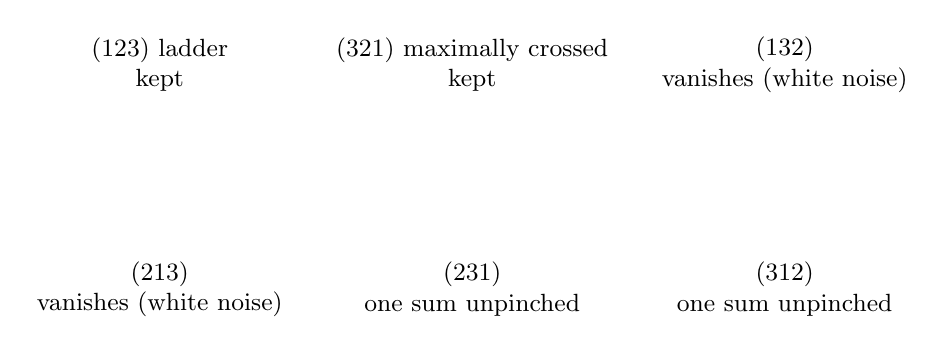
\begin{tikzpicture}[scale=0.62]
 \begin{scope}
  \permdiag{1.0}{2.3}{3.6}
  \node[lab,align=center] at (2.3,-2.6) {$(123)$ ladder\\ kept};
 \end{scope}
 \begin{scope}[xshift=6.4cm]
  \permdiag{3.6}{2.3}{1.0}
  \node[lab,align=center] at (2.3,-2.6) {$(321)$ maximally crossed\\ kept};
 \end{scope}
 \begin{scope}[xshift=12.8cm]
  \permdiag{1.0}{3.6}{2.3}
  \node[lab,align=center] at (2.3,-2.6) {$(132)$\\ vanishes (white noise)};
 \end{scope}
 \begin{scope}[yshift=-4.6cm]
  \permdiag{2.3}{1.0}{3.6}
  \node[lab,align=center] at (2.3,-2.6) {$(213)$\\ vanishes (white noise)};
 \end{scope}
 \begin{scope}[xshift=6.4cm,yshift=-4.6cm]
  \permdiag{2.3}{3.6}{1.0}
  \node[lab,align=center] at (2.3,-2.6) {$(231)$\\ one sum unpinched};
 \end{scope}
 \begin{scope}[xshift=12.8cm,yshift=-4.6cm]
  \permdiag{3.6}{1.0}{2.3}
  \node[lab,align=center] at (2.3,-2.6) {$(312)$\\ one sum unpinched};
 \end{scope}
\end{tikzpicture}
\caption{The $3!=6$ ways of joining three rungs between the
retarded line (top) and the advanced line (bottom), labelled by
$\pi=(\pi(1)\pi(2)\pi(3))$. The ladder arrangement has equal
retarded and advanced momenta between rungs, while the maximally
crossed arrangement has opposite momenta in the
$\mathbf K\to0$ limit; both retain the retarded--advanced
enhancement. The two mixed arrangements retain it too but
vanish for white noise; the last two lose one pinched sum.}
\label{fig:perm}
\end{figure}

% ===== Figure: arc crossing a rung =====
\begin{figure}[ht]
\centering
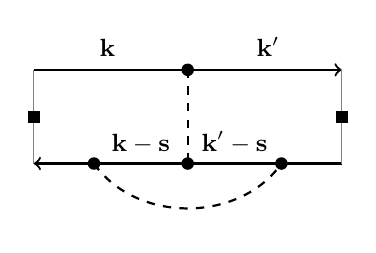
\begin{tikzpicture}[scale=0.85]
 \draw[ret] (0,0)--(4.6,0);
 \draw[adv] (0,-1.4)--(4.6,-1.4);
 \draw[gray] (0,0)--(0,-1.4);
 \draw[gray] (4.6,0)--(4.6,-1.4);
 \node[vert] at (0,-0.7) {};
 \node[vert] at (4.6,-0.7) {};
 \node[dot] at (2.3,0) {};
 \foreach \x in {0.9,2.3,3.7}{
  \node[dot] at (\x,-1.4) {};
 }
 \draw[imp] (2.3,0)--(2.3,-1.4);
 \draw[imp] (0.9,-1.4) to[bend right=55] (3.7,-1.4);
 \node[lab,above] at (1.1,0.05) {$\mathbf k$};
 \node[lab,above] at (3.5,0.05) {$\mathbf k'$};
 \node[lab,above] at (1.6,-1.4) {$\mathbf k-\mathbf s$};
 \node[lab,above] at (3.0,-1.4) {$\mathbf k'-\mathbf s$};
\end{tikzpicture}
\caption{An arc crossing a rung ($N=4$). The advanced
propagators inside the arc carry $\mathbf k-\mathbf s$ and
$\mathbf k'-\mathbf s$ with $\mathbf s$ summed freely, so the
loop contains two advanced functions and no retarded--advanced
pair: it is not leading.}
\label{fig:straddle}
\end{figure}


\subsection*{B.5\quad The dressed bubble and the sum of the diagrams}

\paragraph{Dressed bubble.}
With no rung the pairings on the two lines are independent and
their sum factorises,
$\overline{G^RG^A}\to\overline G^R\,\overline G^A$.
Closing the two dressed lines into a loop with the two current
vertices gives the \emph{dressed bubble}
(Fig.~\ref{fig:bubble}),
\[
S^{(0)}
=\sum_{\mathbf k}v_{\mathbf k x}^2\,
\overline G^R(\mathbf k)\,
\overline G^A(\mathbf k),
\]
with one momentum summed. This is class~1. The bare bubble of
$g_0^Rg_0^A$ alone is not meaningful, since
$\int\mathrm{d}\xi\,g_0^Rg_0^A=\pi/0^+$ diverges; the arcs
supply the finite width $\gamma$.

% ===== Figure 3: the bubble, bare and dressed =====================
\begin{figure}[ht]
\centering
\begin{tikzpicture}[scale=0.85]
 % loop of exact lines (left)
 \draw[ret] (0,0)--(4.4,0);
 \draw[adv] (0,-1.4)--(4.4,-1.4);
 \draw[gray] (0,0)--(0,-1.4);
 \draw[gray] (4.4,0)--(4.4,-1.4);
 \node[vert] at (0,-0.7) {};
 \node[vert] at (4.4,-0.7) {};
 \node[lab,left] at (-0.15,-0.7) {$v_x$};
 \node[lab,right] at (4.55,-0.7) {$v_x$};
 \node[lab,above] at (2.2,0.08) {$G^R$};
 \node[lab,below] at (2.2,-1.45) {$G^A$};
 \node[lab] at (2.2,-2.6) {exact lines of one sample};
 \node at (6.9,-0.7) {$\xrightarrow{\ \text{average}\ }$};
 % dressed bubble (right)
 \begin{scope}[xshift=9.4cm]
  \draw[thickline] (0,0)--(4.4,0);
  \draw[thickadv] (0,-1.4)--(4.4,-1.4);
  \draw[gray] (0,0)--(0,-1.4);
  \draw[gray] (4.4,0)--(4.4,-1.4);
  \node[vert] at (0,-0.7) {};
  \node[vert] at (4.4,-0.7) {};
  \node[lab,left] at (-0.15,-0.7) {$v_x$};
  \node[lab,right] at (4.55,-0.7) {$v_x$};
  \node[lab,above] at (2.2,0.08) {$\overline G^R(\mathbf k)$};
  \node[lab,below] at (2.2,-1.45) {$\overline G^A(\mathbf k)$};
  \node[lab] at (2.2,-2.6) {dressed bubble (class 1)};
 \end{scope}
\end{tikzpicture}
\caption{The retarded line (top, arrow to the right) and the
advanced line (bottom, arrow to the left) are joined by two
current vertices to form the loop that appears in the
conductivity. After averaging, all arcs on a single line are
absorbed into the thick (dressed) propagators; the loop of two
thick lines with no dashed line between them is the dressed
bubble, class~1.}
\label{fig:bubble}
\end{figure}

\paragraph{Bubbles with rungs.}
Adding $n$ rungs gives the other families. For the ladder
(identity arrangement) the two lines carry the same momentum
between rungs, so with the momenta
$\mathbf p_0,\dots,\mathbf p_n$ of the $n+1$ dressed pairs and
a weight $W_0/V$ per rung,
\[
S^{(n)}_{\mathrm{ladder}}
=
\left(\frac{W_0}{V}\right)^n
\sum_{\mathbf p_0,\dots,\mathbf p_n}
v_{\mathbf p_0x}
\left[
\prod_{j=0}^{n}
\overline G^R(\mathbf p_j)
\overline G^A(\mathbf p_j)
\right]
v_{\mathbf p_nx}.
\]
For the maximally crossed arrangement (reversal) the advanced
momenta are $\mathbf K-\mathbf p_j$ with
$\mathbf K=\mathbf k+\mathbf k'$ the same at every rung; this
family, $S^{(n)}_{\mathrm{cross}}$ with $n\ge2$, is written out
in the main text.

\paragraph{The sum.}
The averaged retarded--advanced trace is therefore the sum of
the leading families (Fig.~\ref{fig:sum}),
\[
\begin{aligned}
\overline{\operatorname{Tr}[v_xG^Rv_xG^A]}
\simeq{}&
\underbrace{S^{(0)}}_{\text{class 1}}
+\underbrace{\sum_{n\ge1}S^{(n)}_{\mathrm{ladder}}}
_{\text{class 2}}\\
&+
\underbrace{\sum_{n\ge2}S^{(n)}_{\mathrm{cross}}}
_{\text{class 3}},
\end{aligned}
\]
where $\simeq$ means that the arrangements that fail the pinch
rule of B.4 are dropped. By the Kubo--Greenwood formula of
Appendix~A, in which the retarded--advanced term carries the
prefactor $e^2g_s/2\pi V$, this is the conductivity:
\[
\begin{aligned}
\sigma_{dc}
&\simeq
\frac{e^2g_s}{2\pi V}
\left[
S^{(0)}
+\sum_{n\ge1}S^{(n)}_{\mathrm{ladder}}
+\sum_{n\ge2}S^{(n)}_{\mathrm{cross}}
\right]\\
&=\sigma_D+\delta\sigma_{\mathrm{WL}}.
\end{aligned}
\]
Class~1 is the bubble of independently dressed lines, the
Drude-type term; class~2 adds the vertex corrections of the
ladder; together they give the Drude conductivity
$\sigma_D$ for the isotropic white-noise model used here, where
the ladder correction to the uniform current vertex vanishes
(Appendix~C); this is not a universal statement for arbitrary
disorder. Class~3 is the interference of an electron path with
its time-reversed partner and gives the correction
$\delta\sigma_{\mathrm{WL}}$ (main text). The terms of the
same-side type, RR and AA, are left out here (Appendix~C).

% ===== Figure: the sum of diagrams in the retarded-advanced bubble ==
\begin{figure}[ht]
\centering
\begin{tikzpicture}[scale=0.52]
 \tikzset{tl/.style={very thick,->},ta/.style={very thick,<-}}
 \newcommand{\frm}{
   \draw[tl] (0,0)--(4.6,0);
   \draw[ta] (0,-1.4)--(4.6,-1.4);
   \draw[gray] (0,0)--(0,-1.4);
   \draw[gray] (4.6,0)--(4.6,-1.4);
   \node[vert] at (0,-0.7) {};
   \node[vert] at (4.6,-0.7) {};
 }
 % ---- row 1
 \begin{scope}
  \frm
  \node[lab] at (2.3,-2.4) {dressed bubble};
  \node at (5.6,-0.7) {$+$};
 \end{scope}
 \begin{scope}[xshift=6.6cm]
  \frm
  \node[dot] at (2.3,0) {};
  \node[dot] at (2.3,-1.4) {};
  \draw[imp] (2.3,0)--(2.3,-1.4);
  \node[lab] at (2.3,-2.4) {one rung};
  \node at (5.6,-0.7) {$+$};
 \end{scope}
 \begin{scope}[xshift=13.2cm]
  \frm
  \foreach \x in {1.5,3.1}{
   \node[dot] at (\x,0) {};
   \node[dot] at (\x,-1.4) {};
   \draw[imp] (\x,0)--(\x,-1.4);
  }
  \node[lab] at (2.3,-2.4) {two rungs};
  \node at (5.6,-0.7) {$+\cdots$};
 \end{scope}
 % ---- row 2
 \begin{scope}[yshift=-4.2cm]
  \frm
  \node[dot] at (1.5,0) {};
  \node[dot] at (3.1,0) {};
  \node[dot] at (1.5,-1.4) {};
  \node[dot] at (3.1,-1.4) {};
  \draw[imp] (1.5,0)--(3.1,-1.4);
  \draw[imp] (3.1,0)--(1.5,-1.4);
  \node[lab] at (2.3,-2.4) {two crossed rungs};
  \node at (5.6,-0.7) {$+$};
 \end{scope}
 \begin{scope}[xshift=6.6cm,yshift=-4.2cm]
  \frm
  \foreach \x in {1.1,2.3,3.5}{
   \node[dot] at (\x,0) {};
   \node[dot] at (\x,-1.4) {};
  }
  \draw[imp] (1.1,0)--(3.5,-1.4);
  \draw[imp] (2.3,0)--(2.3,-1.4);
  \draw[imp] (3.5,0)--(1.1,-1.4);
  \node[lab] at (2.3,-2.4) {three crossed rungs};
  \node at (5.6,-0.7) {$+\cdots$};
 \end{scope}
\end{tikzpicture}
\caption{The retarded--advanced bubble organised into families
(thick lines are dressed propagators). Top row: the dressed
bubble (class~1) and the ladder with one, two, \dots{}
uncrossed rungs (class~2). Bottom row: the maximally crossed
diagrams with two, three, \dots{} rungs (class~3). Arcs that do
not cross a rung are already inside the thick lines
(Sec.~B.4). The other rung patterns are discussed in
Sec.~B.4 and Fig.~\ref{fig:perm}.}
\label{fig:sum}
\end{figure}